\section{Cat pictures}
\label{sec:cats}
% Labelling a section lets us refer to it from other places in the document.

Cat pictures are a great teaching aid \citep{smith2016}. % A parenthesised citation.

\citet{smith2016} says every \LaTeX\ presentation should begin with a cat picture. % An in-text citation.

Use a command provided by graphicx to add a picture:


\includegraphics{figures/cat.jpg}

Use an option in square brackets to change the image width:


\includegraphics[width=0.9\textwidth]{figures/cat.jpg}

Note that Figure~\ref{fig:cat-picture-1} is inside a figure environment
defined like so:

\begin{verbatim}
\begin{figure}
    \begin{center}
        
\includegraphics{figures/cat.jpg}
        \caption{Meow!}
        \label{fig:cat-picture-1}
    \end{center}
\end{figure}
\end{verbatim}

This lets LaTeX float the image to a spot where it will look reasonably tidy.

At first this can take some getting used to because the figure in the final
PDF will often not appear right where you specify it in the \LaTeX\ source.
In fact, if you have it set in your mind that an image
must appear at an exact point you specify, \LaTeX\ will
seem wilfully frustrating.
People can get quite irate when they think they know how their document
should look, only to find that \LaTeX\ stubbornly disagrees.

To avoid frustration, try to train yourself to trust
that \LaTeX\ knows what it's doing.
It was, after all, written with beautiful typesetting as its highest priority.
To stick to best practice, put each image inside a figure environment,
with a label, and then rather than saying ``see the following image:'',
say ``see Figure~\ref{fig:cat-picture-1}''.

\begin{figure}
    \begin{center}
        
\includegraphics{figures/cat.jpg}
        \caption{Meow!}
        \label{fig:cat-picture-1}
    \end{center}
\end{figure}

Note that other types of floating environments are available, such as for tables.

Also note that when including mathematical or technical diagrams,
it's often prettier and easier to manage if you create them
directly in your \LaTeX\ document rather than including a pre-rendered image.

\begin{figure}
    \begin{center}
        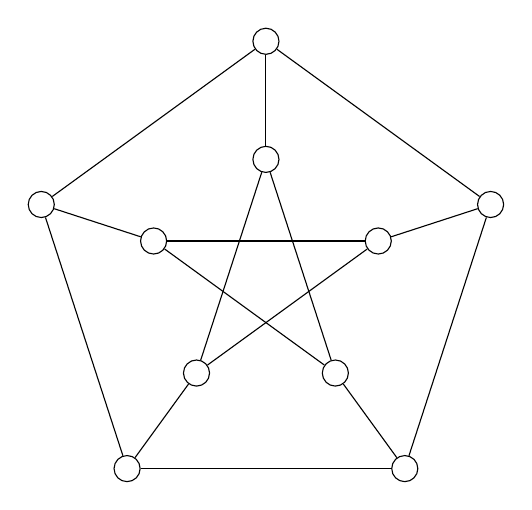
\begin{tikzpicture}
            \node (inner1) at (90:1.5) [shape=circle,draw] {};
            \node (inner2) at (162:1.5) [shape=circle,draw] {};
            \node (inner3) at (234:1.5) [shape=circle,draw] {};
            \node (inner4) at (306:1.5) [shape=circle,draw] {};
            \node (inner5) at (18:1.5) [shape=circle,draw] {};
            \node (outer1) at (90:3) [shape=circle,draw] {};
            \node (outer2) at (162:3) [shape=circle,draw] {};
            \node (outer3) at (234:3) [shape=circle,draw] {};
            \node (outer4) at (306:3) [shape=circle,draw] {};
            \node (outer5) at (18:3) [shape=circle,draw] {};
            \draw (inner1)--(inner3);
            \draw (inner1)--(inner4);
            \draw (inner2)--(inner4);
            \draw (inner2)--(inner5);
            \draw (inner3)--(inner5);
            \draw (inner1)--(outer1);
            \draw (inner2)--(outer2);
            \draw (inner3)--(outer3);
            \draw (inner4)--(outer4);
            \draw (inner5)--(outer5);
            \draw (outer1)--(outer2);
            \draw (outer2)--(outer3);
            \draw (outer3)--(outer4);
            \draw (outer4)--(outer5);
            \draw (outer5)--(outer1);
        \end{tikzpicture}
        \caption{Petersen graph}
        \label{fig:petersen}
    \end{center}
\end{figure}

Figure~\ref{fig:petersen} requires you to use tikz-pgf
\citep{tantau-tikz-pgf-3.0.1a}.
This is a general purpose package for drawing diagrams
within a \LaTeX\ document.
There are also packages specifically for things like
commutative diagrams, Feynman diagrams, and musical scores.
However, tikz is general purpose, powerful, and widespread enough
that it will cover most scenarios.
